\chapter{Wikipedia}
\label{chp:wikipedia}
In this chapter, we provide an overview of the inner workings and decision making processes of Wikipedia. Firstly, in Section~\ref{sec:principles-wikipedia} we state the fundamental principles of Wikipedia and how it guides editors on the website. Next, we describe the roles and responsibilities of the  different categories of Wikipedia users in Section~\ref{sec:formal-org-wikipedia}. Lastly, we explain the election process for administrators and discuss the voting behaviour in terms of existing research. 

\section{Principles of Wikipedia}
\label{sec:principles-wikipedia}
Wikipedia is the largest online encyclopedia with over six million pages of content in the English version. It is maintained by an open collaborative effort of multiple editors from all across the world. All the knowledge and content is free and is supported by the non-profit Wikimedia Foundation. The size and popularity of Wikipedia is attributed to the ability for anyone to edit any content. All editors on Wikipedia follow five fundamental principles called the "Five Pillars" shown in Figure~\ref{fig:5-pillars}. It provides a foundational framework for collaboration and contribution to the Wikipedia project.   
\begin{figure}[!ht]
    \centering
    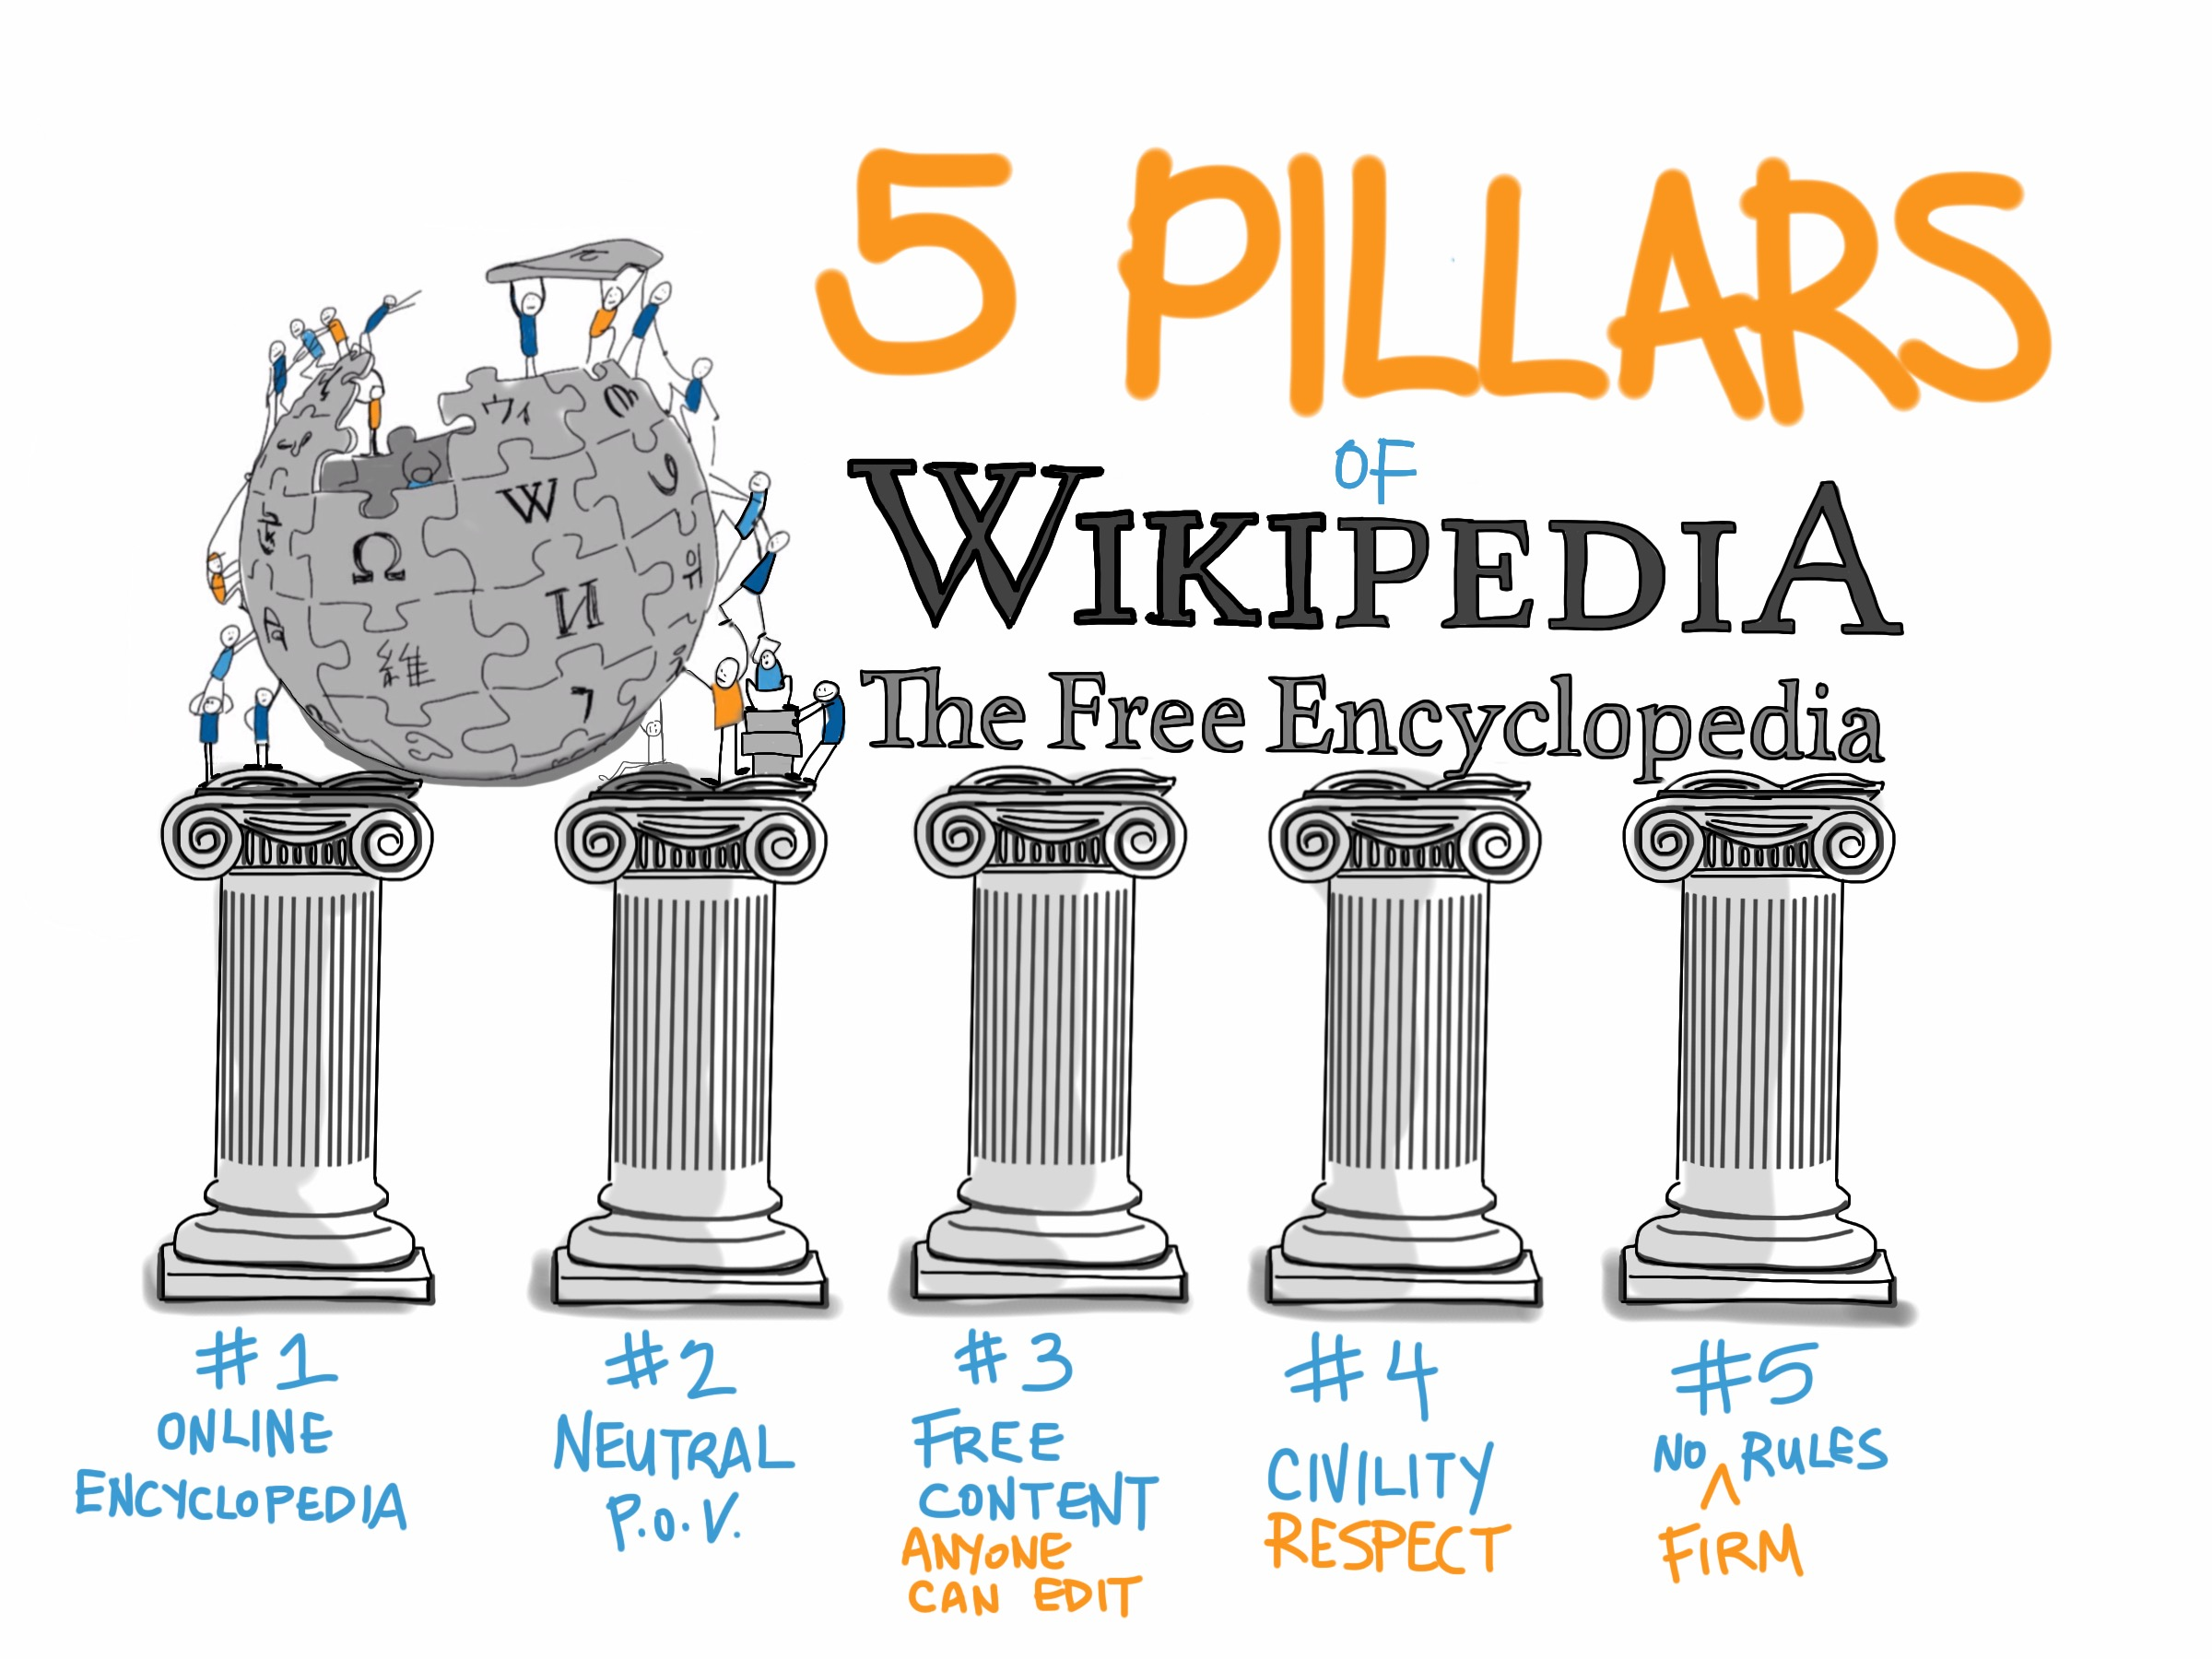
\includegraphics[width=0.75\textwidth]{images/Pillars.jpg}
    \caption{Five Pillars of Wikipedia. Image downloaded from \url{https://www.flickr.com/photos/gforsythe/21684596874}}
    \label{fig:5-pillars}   
\end{figure}

The first pillar states that Wikipedia is first and foremost an encyclopedia \cite{wiki:wiki-is-not}. Therefore, it must strictly not contain any original research, propaganda or advertisements \cite{wiki:wiki-NOR}. Materials that do not have reliable references will be removed by other edits.

The second pillar describes that articles on Wikipedia should strive to have a neutral point of view. This might include presenting multiple perspectives on the same subject accurately and not championing any one viewpoint as "correct" or "the truth". If disagreements are present then discussions must take place for building consensus.

The third principle enshrines the ideal that all content available on Wikipedia is free to edit and share. However, this does not mean copyrights and plagiarism is tolerated by the community. There is no ownership of an article by an editor; anyone may freely modify any content.

The fourth pillar describes Wikipedia's code of conduct. It asks users to act in good faith and assume good faith on the part of other editors. Wikipedia etiquette urges disputes and disagreements such as edit wars \cite{wiki:edit-wars}, to be resolved with civility while respecting other editors.

The fifth and last pillar reminds users that all rules in Wikipedia are policies and guidelines meant to help with collaboration. They can evolve and change to reflect the requirement of the community. It assuages the fear of making mistakes and encourages editors to be bold though not reckless. 

\section{Formal Organization of Wikipedia}
\label{sec:formal-org-wikipedia}
\subsection{Editors}
\subsection{Administrators}
\subsection{Bureaucrats}
\subsection{Arb Committee}

\section{Request for Adminship}
\begin{itemize}
    \item Describe the Request for Administrator(RfA) process
    \item Discuss general trends and patters
    \item Mention research interest and possible current works?
\end{itemize}

\subsection{Existing Research}